\documentclass[answers,addpoints,12pt]{exam}
\usepackage{multicol,xy}
\usepackage{graphicx,multicol}
\usepackage[euler-digits]{eulervm}
\usepackage{charter,amsmath,amssymb}
\usepackage[letterpaper,margin=1in]{geometry}
\pagestyle{headandfoot}
\runningheadrule
\firstpageheader{\bf Math 104}{\bf Exam 3, Red Form}{\bf 29 October 2014}
\runningheader{\bf Math 104}
{\bf Exam Three, Page \thepage\ of \numpages}
{\bf 29 October 2014}
\firstpagefooter{}{}{}
\runningfooter{}{}{}
\everymath{\displaystyle}
\begin{document}

\begin{center}
\fbox{\fbox{\parbox{5.5in}{
This exam has \numquestions~questions.
It has been printed on \numpages~pages and is worth \numpoints~points.
Answer all the questions below in the spaces provided.
In order to receive maximum credit, you must
clearly indicate how you arrived at your answers.
By signing below, you pledge that you
\begin{enumerate}
\item will not communicate to any person in any conceivable way anything
about the contents of this exam
until all students have taken the exam, and
\item in taking this exam now,
you have not been the recipient of such communication from anyone else.
\end{enumerate}}}}
\end{center}
\vspace{.2in}
\makebox[\textwidth]{Your signature:\enspace\hrulefill}\\
\vspace{.2in}\\
\makebox[\textwidth]{Your name:\enspace\hrulefill}\\
\vspace{.2in}\\
\makebox[\textwidth]{Your student ID number:\enspace\hrulefill}\\

\begin{questions}
\question The following table lists
the languages other than English spoken by residents
of Iowa between 2008 and 2012, organized by the age
of the resident.\footnote{Source: {\tt www.census.gov}}
\[\begin{array}{r|rrr|r}
\text{Language}&\text{$5$--$17$}
&\text{$18$--$64$}&\ge 65&\text{Total}\\\hline
\text{Spanish or Spanish Creole}&32,196&75,674&4,114&111,984\\
\text{Other Indo-European}&8,978&29,811&6,530&45,319\\
\text{Asian or Pacific Island}&5,624&27,022&2,255&34,901\\
\text{Other}&2,386&7,874&423&10,683\\\hline
\text{Total}&49,184&140,381&13,322&202,887
\end{array}\]
\begin{parts}
\part How many residents of age $65$ and older
spoke a language other than English?
\part What is the probability that a randomly selected
resident spoke an Asian or Pacific Island language
given that that individual was between $18$ and $64$ years old?
\part What is the probability that a randomly selected
resident that spoke a language other than English
was between $5$ and $17$ years old?
\end{parts}

\question Two cards are drawn at random from a deck of playing cards
without replacement.
\begin{parts}
\part What is the probability that both cards are kings?
\part What is the probability that the second card is a King
given that the first card is a Queen?
\end{parts}
\begin{solution}
\begin{parts}
\part $\frac{4}{52}\cdot\frac{3}{51}=\frac{1}{221}
\approx 0.005$
\part $\frac{4}{51}\approx 0.078$
\end{parts}
\end{solution}

\begin{multicols}{2}
\question
New Jersey license plates contain a letter,
followed by two digits, followed by three letters,
as illustrated in the image at the right.
How many license plates in New Jersey are possible?\\
\columnbreak
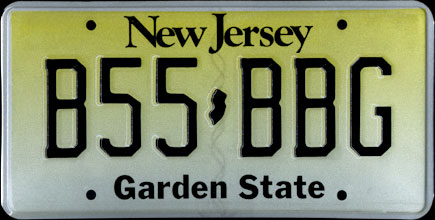
\includegraphics[scale=.3]{NewJersy}
\end{multicols}
\begin{solution}
$26\cdot 10\cdot 10\cdot 26\cdot 26\cdot 26=26^4\cdot 10^2
=45,697,600$
\end{solution}

\question How many anagrams of the word
{\textsf{Machiavellianism}} are there?
\begin{solution}
The number of times each distinct letter appears is
shown in the following table.
\[\begin{array}{r|cccccccccc}
\text{letter}&a&c&e&h&i&l&m&n&s&v\\\hline
\text{frequency}&3&1&1&1&3&2&2&1&1&1
\end{array}\]
Thus the number of anagrams is
\[\frac{16!}{3!3!2!2!}=145,297,152,000.\]
\end{solution}

\question In a recent survey of 884 Americans between the ages
of $18$ and $50$, $120$ reported that they have tattoos,
$72$ have body piercings, and $41$ have both.
\footnote{2004, American Journal of Dermatology}
\begin{parts}
\part What is the probability that a randomly
selected American has a tattoo?
\part What is the probability that a randomly
selected American has a piercing?
\part What is the probability that a randomly
selected American has a both a tattoo and a piercing?
\part\label{Independent} According to this data do
the decision to get a piercing and the decision
to get a tattoo appear to be independent?
\part Does your response to part~(\ref{Independent}) make
sense in this context?
\part What is the probability that a randomly
selected American has a tattoo given that that individual
has a piercing?
\part What is the probability that a randomly
selected American has a piercing given that that individual
does {\bf not} have a piercing?
\end{parts}

\question Suppose $E=\left\{a,c,d,e,f\right\}$,
$F=\left\{b,c,g,h,i\right\}$, and $G=\left\{a,b,e,h,i\right\}$.
\begin{parts}
\part Calculate $\left(E\cup G\right)\cap\left(F\cup G\right)$
\part Calculate $\left(E\cap F\right)\cup G$
\end{parts}
\begin{solution}
\begin{align*}
E\cup G&=\left\{a,b,c,d,e,f,h,i\right\}\\
F\cup G&=\left\{a,b,c,e,g,h,i\right\}\\
\text{so}\quad
\left(E\cup G\right)\cap\left(F\cup G\right)
&=\left\{a,b,c,e,h,i\right\}\\
E\cap F&=\left\{c\right\}\\
\text{so}\quad\left(E\cap F\right)\cup G
&=\left\{a,b,c,e,h,i\right\}
\end{align*}
\end{solution}
\end{questions}
\end{document}
